\section{Methodology}
\noindent
For any time series, two characteristics are attributed to each event: occurrence time and value of the event. Two events are in connection or visible to each other if no other event interrupts their linear connection. In mathematical form, events $i$ and $j$ are visible to each other if the following equation is fulfilled:

\begin{equation}
\frac{y_i - y_k }{t_k - t_i} > \frac{y_i - y_j}{ t_j - t_i} ,
\end{equation}
\noindent
where $y$ is the value and $t$ is the time of the event, and $k$ is the index of any event occurring between events  $i$  and  $j$. The visibility graph generated from a time series holds the following conditions: 1) each event is visible to the first event at its right and left side (if there is any) (Connectivity); 2) the algorithm is developed without defining a direction for the links (Undirected); and 3) rescaling or translation of a time series does not change the resulting visibility graph (invariant under affine transformations of the series data) \citep{Lacasa2008}. 
\noindent
For each seismic event we calculate the connectivity degree $(K)$. The connectivity degree of each event is sum of all connections of the event with the visible events. We categorized events in small magnitude bins $(\Delta M=0.1)$ and plot connectivity degree as a function of the bin-magnitude. Two earthquakes with the same magnitude could have different connectivity degrees, based on event time and surrounding events. We compute the linear regression line for scatter data points. The slope of the line is $k-M$ slope of the time series. Fig.~\ref{fig:vg} shows initial events of KopehDagh magnitude-time series with connectivity degree of each event. 

\begin{figure} [ht]
\centering
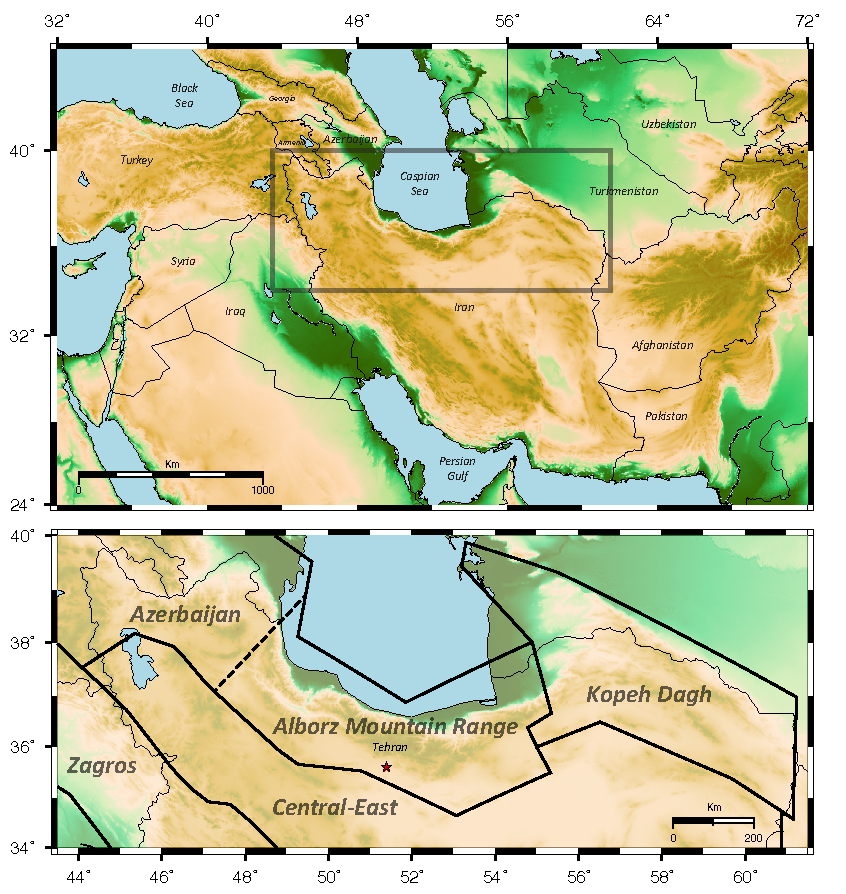
\includegraphics[scale=0.24]{figures/pdf/Figure01.pdf} 
\caption{Sketch of the VG method. The initial events of Kopeh Dagh region are represented. Couple of events were deleted due to illustration purposes. The blue vertical lines indicate the events. Height of each line is corresponding the magnitude of the event. The green dashed lines show the allowable connections between events. The connectivity degree (K) of each event is presented. The red arrows show the time difference between events. The $T_c$ and $< T_c >$ values of the last event are represented. Note that the mean of all $<T_c>$ values in each window will be the window mean interval connectivity time.}
\label{fig:vg}
\end{figure}
\noindent
\citet{Telesca2014} defined the VG window mean interval connectivity time $<T_c>$ as an indication of mean linkage time between earthquakes. For each event in a window we compute the interval connectivity time $(T_c)$ for each connection which is the time difference between occurrence of two events. Average interval connectivity time gives the mean interval connectivity time $<T_c>$  for each event. The average of all the $<T_{ce}>$  values in a window results the window mean connectivity time $<T_c>$. We attribute this value to the last event in each window. Fig.~\ref{fig:vg} shows the  $T_c$ and $< T_c >$ values of the last event. 